\documentclass[border=10pt]{standalone}
\usepackage{tikz}

\begin{document}
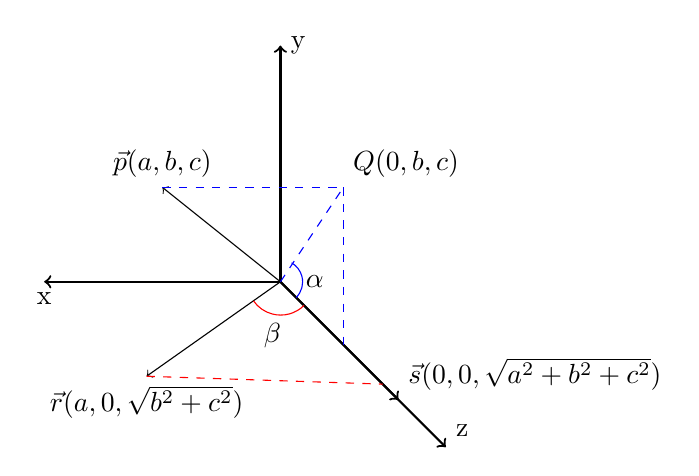
\begin{tikzpicture}
 
  \coordinate (O) at (0,0);
  \coordinate (X) at (-3,0);
  \coordinate (Y) at (0,3);
  \coordinate (Z) at (2.1,-2.1);
  
  \draw [->][thick] (O) -- (X) node [below] {x};
  \draw [->][thick] (O) -- (Y) node [right] {y};
  \draw [->][thick] (O) -- (Z) node [above right] {z};
  
  
  \coordinate (P) at (-1.5, 1.2);
  \coordinate (Q) at (0.8, 1.2);
  \coordinate (QZ) at (0.8, -0.8);
  \coordinate (R) at (-1.7, -1.2);
  \coordinate (RZ) at (1.3, -1.3);
  \coordinate (S) at (1.5, -1.5);
  
  \draw [->] (O) -- (P);
  \draw [->] (O) -- (R);
  \draw [->][thick] (O) -- (S);
  
  \draw [blue, dashed] (O) -- (Q);
  \draw [blue, dashed] (P) -- (Q);
  \draw [blue, dashed] (Q) -- (QZ);
  \draw [red, dashed] (R) -- (RZ);
  
  \node [above] at (P) {$\vec{p}(a,b,c)$};
  \node [above right] at (Q) {$Q(0,b,c)$};
  \node [below] at (R) {$\vec{r}(a,0,\sqrt{b^2+c^2})$};
  \node [above right] at (S) {$\vec{s}(0,0,\sqrt{a^2+b^2+c^2})$};
  
  
  % label \alpha and \beta
  \coordinate (AS) at (0.2, -0.2);
  \coordinate (BS) at (0.3, -0.3);
  \coordinate (AL) at (0.2, -0.0);
  \coordinate (BL) at (-0.1, -0.4);
  
  \draw [blue] (AS) arc [x radius=0.28, y radius=0.28, start angle=-45, end angle=60];
  \draw [red] (BS) arc [x radius=0.42, y radius=0.42, start angle=-45, end angle=-145];
  \node [right] at (AL) {$\alpha$};
  \node [below] at (BL) {$\beta$};
 
\end{tikzpicture}
\end{document}
